\chapter{Ergebnisse}
\label{ch:ergebnisse}

\section{Analyse des LSS- und LSR-Formates}

In der Online-Dokumetation von LimeSurvey gibt es zwar eine Sektion zum Thema Export und Export-Formate, der Abschnitt war aber bis vor kurzem leer.
Auch jetzt enthält das Kapitel nur eine oberflächliche Beschreibung der Formate, die genaue Struktur wird nicht erklärt.
Da diese allerdings benötigt wird, um eine Konvertierung vornehmen zu können, muss zunächst ermittelt werden, wie die .lss- und .lsr-Dateien genau aufgebaut sind.

Dies wurde bewerkstelligt, indem zunächst eine simple Umfrage erstellt wurde, welches eine Fragegruppe und drei Freitextfragen enthält.
Dafür wurde eine Instanz der LimeSurvey Community Edition benötigt, diese aufzusetzen war dank existierenden Docker-Compose-Dateien relativ simpel.

Nachdem die Struktur der Umfrage selbst, sowie der Fragegruppen so ermittelt werden konnte, wurden komplexere Dateien erstellt.
Diese enthielten zunächst Fragen mit festen Antwortmöglichkeiten, also vor allem Maskenfragen und Multiple Choice Fragen.
Nachdem so auch die Struktur der Antworten deutlich geworden war, wurden zuletzt die Matrixfragen eingebaut und die Struktur der Subfragen ermittelt.
Zuletzt wurden Anzeigebedingungen in die Umfragen eingebracht und deren Struktur ermittelt.

Das Ergebis dieser Analyse wird im Folgenden dargestellt (Es werden nicht alle existierenden Elemente angesprochen, sondern nur die für diese Arbeit relevanten, eine vollständige Auflistung kann im \cref{app:lss} gefunden werden):

\subsection{Grundlegende Struktur}

Das Wurzel-Element in LSS ist \el{document}.
Hier sind zuerst grundlegende Informationen wie die Datenbank-Version und den Typ des Dokuments enthalten.
Jedes der größeren direkten Kind-Elemente in \el{document} hat die gleiche Struktur.
Es gibt dort zwei Kind-Elemente, \el{fields} und \el{rows}. In \el{rows} gibt es \el{row} Elemente, welche die Informationen selbst in weiteren Elementen enthalten.
In \el{fields} gibt es \el{fieldname} Elemente, wobei es für jedes mögliche Kind-Element von \el{row} ein \el{fieldname} Element mit dem Namen des Kindelements als Text gibt.
In den Feldern werden also einmal alle Elemente genannt, die sich innerhalb einer Reihe befinden können.

\subsection{Fragegruppen}

Im Element \el{groups} werden Metadaten über Fragegruppen gesammelt, wie zum Beispiel die Gruppen-ID.
Diese sind aber auch in \el{group\_l10ns} enthalten, darüber hinaus finden sich auch noch weitere Inhalte wie Gruppenname und Sprache in diesem Element.
Daher werden später keine Informationen aus \el{groups} verwendet.
Ein \el{row} Element steht hier für eine Fragegruppe.

\subsection{Fragen}

Das Element \el{questions} enthält Metadaten über Fragen, wie \el{qid}, \el{gid}, \el{title} und \el{type}.
Ein \el{row} Element steht hier für eine Frage, pro \enquote{Haupt}-Frage in der Umfrage gibt es ein Element in \el{questions}.
\el{subquestions} enthält Subfragen von Arrays, Matrizen et cetera. Diese sind via \el{parent\_qid} an ein Element aus \el{questions} gekoppelt.
Auch in \el{subquestions} sind nur Metadaten enthalten, jede Subfrage hat, wie die \enquote{Haupt}-Fragen auch, eine Fragen-ID.

In \el{question\_l10ns} gibt es nun die tatsächliche Frage in \el{question}, ein Element innerhalb einer Reihe.
Weiterhin gibt es mit \el{help} einen Hilfstext für die Frage, \el{language} gibt die Sprache des Fragetextes an.
Für jedes Element aus \el{question} und \el{subquestion} gibt es hier ein Element pro Sprache.
Referenziert werden diese mit der \el{qid}.

\el{question\_attributes} enthält Informationen über eine Frage wie ein Prä-/Suffix zu der Antwort, RegEx-Validations-Ausdrücke für die Antwort, Timings und Informationen zur Darstellung einer Frage (Textfeldbreite, Default-Antworten).

\subsection{Antwortmöglichkeiten}

Es gibt eine Reihe an Fragen, für die es eine Menge an vordefinierten Antworten gibt.
Diese sind entweder schon durch die Frage festgelegt, wie bei dem Fragetyp \el{5 Punkte Wahl} oder dem Typ \el{Geschlecht}, oder der Umfrage-Ersteller kann sie selber angeben.
Sind die Möglichkeiten schon durch den Typ festgelegt, werden die Antwortmöglichkeiten implizit ermittelt und nie konkret im LSS-Dokument niedergeschrieben.

Hat der Umfrage-Ersteller die Möglichkeiten selber festgelegt, werden diese in \el{answers} und \el{answer\_l10ns} gespeichert.
In \el{answers} gibt es dabei wieder Metadaten wie \el{qid}, \el{aid}, und einen \el{code}.
In \el{answer\_l10ns} hingegen gibt es den Antworttext in \el{answer}, eine \el{aid} zur Verknüpfung mit den Metadaten und die Sprache in \el{language}.
Für jedes Element aus \el{answers} gibt es pro Sprache ein Element in \el{answer\_l10ns}.

\subsection{Umfrage-Metadaten}
\label{a:survey_meta}

In \el{surveys} findet man Metadaten über die Umfrage, allerdings sind keine davon für die Konvertierung relevant.
Beispiele wären Daten darüber, ob Willkommenstexte angezeigt werden sollen oder ob IP-Adressen der Teilnehmer gespeichert werden sollen.
\el{surveyls\_languagesettings} enthält relevante Informationen wie die \el{surveyls\_id}, den Titel in \el{surveyls\_title} und eine Beschreibung der Umfrage in \el{surveyls\_description}.
\el{themes} und \el{themes\_inherited} enthalten Informationen über die visuelle Darstellung der Umfrage in LimeSurvey.

\subsection{LSR-Aufbau}

Auch für die Antworten wurde die gleiche Strategie wie für die Umfragestruktur verwendet.
Die Ergebnisse sind wie folgt:

Das Wurzel-Element ist wieder \el{Document}, zuerst gibt es wieder einige Metadaten wie der Typ des Dokuments, die Datenbank-Version und die Sprache.
Dann gibt es ein \el{responses} Element, welches dieselbe grundlegende Struktur wie die Elemente in der LSS-Datei besitzt.
Für jeden Teilnehmer der Umfrage gibt es ein Element vom Typ \el{row}.
Dies enthält eine ID, ein Token, das Absendedatum, die Sprache, einen Seed und die Antworten.
Wenn ein Teilnehmer die Umfrage mehrmals ausfüllt, sind die IDs verschieden, die Tokens aber gleich.
Bei den Antworten gibt es für jede Frage bzw. Subfrage ein Element mit folgendem Namensschema: 
\el{\_\{Survey-ID\}X\{GID\}X\{QID\}\{SQID\}?\{ext\}?}, wobei \el{ext} folgendes sein kann (\enquote{other}$\vert$\enquote{comment}).
Man kann bereits am Format sehen, dass es auch für die \enquote{other} und Kommentar-Felder hier eine separate Antwort gibt.

\subsection{Erstellung eines XML-Schemas}
\label{an:xsd}
Da die Struktur der Umfrage nun bekannt ist, wird ein XML-Schema für das LSS-Format erstellt.
Das sorgt einerseits für eine wesentlich bessere Übersicht über den Aufbau, das kann für zukünftige Arbeit nützlich sein.
Andererseits lässt sich dieses Schema später verwenden, um zu überprüfen, ob es sich bei der Eingabedatei um eine valide LSS-Datei handelt.

\section{Mapping}

Da der Aufbau beider Formate nun bekannt ist, muss überlegt werden, wie man beide LimeSurvey-Formate auf ODM abbilden kann. Im Folgenden werden die verschiedenen Teile von LSS nacheinander abgehandelt und es wird erklärt, wie mit überschüssigen Elementen in ODM ungegangen wird.
Der Text wird dabei das Vorgehen beschreiben, die exakten Elementnamen können in den Grafiken nachgesehen werden.

\begin{figure}[h]
			\centering
			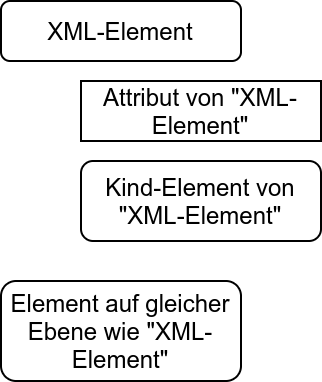
\includegraphics[width=.30\textwidth]{./img/legend.png}
			\caption{Legende für die folgenden Grafiken im Mapping}
\end{figure}

\subsection{Dummy Elemente in ODM}

ODM besitzt mehr Möglichkeiten, die Abläufe einer Studie oder Umfrage darzustellen, da es als generisches Format natürlich mehr Einsatzzwecke abdecken soll, als das LSS-Format.
Dementsprechend gibt es mehrere Wege, LSS auf ODM abzubilden.
Durch die hier getroffenen Entscheidungen werden die Elemente \el{StudyEvent} und \el{GlobalVariables} überflüssig,	da es sich dabei um für eine Studie relevante Felder handelt, es soll aber nur eine Umfrage innerhalb einer Studie erstellt werden.\\

Da diese Elemente dennoch zwingend in ODM vorkommen müssen, werden die globalen Variablen leer gelassen oder mit Dummy-Werten befüllt und es wird ein \el{StudyEvent} erstellt, welches unabhängig von der Eingabe-Datei immer die gleichen Dummy-Werte hat.
Weiterhin wird die \el{OID} des \el{Study} Elements auch auf einen Dummy-Wert gesetzt, da wir hier ebenfalls kein Äquivalent in LSS haben.
Die \el{OID} der \el{MetaDataVersion} soll die Studien-ID behinhalten, da die Version der Metadaten die gesamte Umfrage enthält, es ergibt also Sinn, hier keinen Dummy-Wert einzusetzen sondern eine Referenz auf die Studie mit einzubringen.

\subsection{Umfrage-Eigenschaften}
\label{m:survey_meta}

Innerhalb unseres Dummy-\el{StudyEvent's} gibt es nun ein Formular, dieses soll die Umfrage repräsentieren.
Das \el{Repeating} Attribut wird auf \enquote{No} gesetzt, da die Umfrage nur einmal pro Teilnehmer ausgefüllt werden soll.
Füllt ein Teilnehmer die Umfrage mehrmals aus, gilt das als zwei verschiedene Teilnehmer.
Da das Formular die Umfrage repräsentiert, sollen sie dieselbe ID nutzen, als \el{Name} wird der Titel der Umfrage gesetzt. Die Beschreibung wird ebenfalls in das Formular übernommen.

\subsection{Fragegruppen}
\label{m:qg}
Fragegruppen in LimeSurvey sind fast äquivalent zu \el{ItemGroup's} in ODM.
Entsprechend wird für jede Fragegruppe eine \el{ItemGroupDef} erstellt, die ID wird direkt in ODM übernommen, der Titel wird als Name verwendet, die Beschreibung kann ebenfalls direkt übernommen werden.
Das Attribut \el{Repeating} wird wieder auf \enquote{No} gesetzt.
Entsprechende Referenzen auf die Fragegruppen werden zum Formular hinzugefügt.

\begin{figure}[h]
	\makebox[\linewidth][c]{%
		\begin{subfigure}[b]{.6\textwidth}
			\centering
			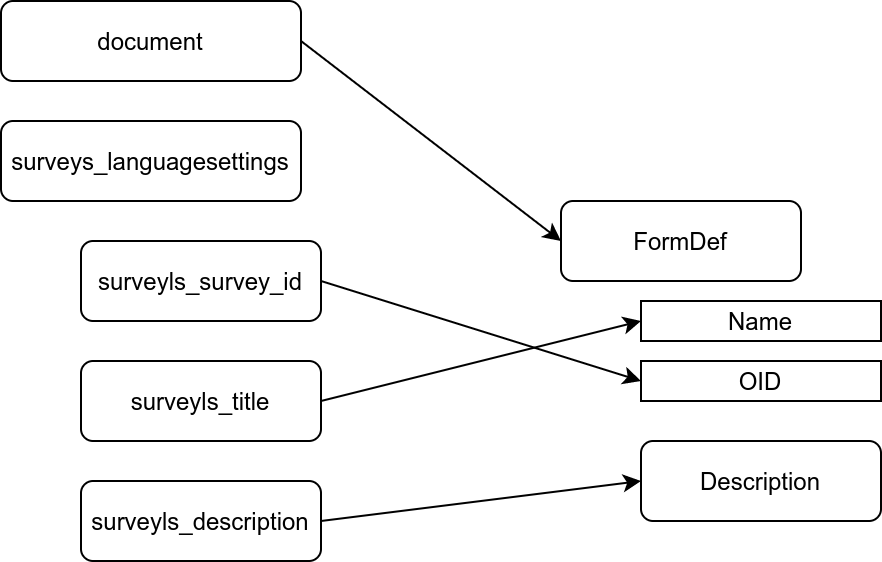
\includegraphics[width=.95\textwidth]{./img/m_survey_props.png}
			\caption{Mapping der Umfrage-Eigenschaften}
		\end{subfigure}%
		\begin{subfigure}[b]{.6\textwidth}
			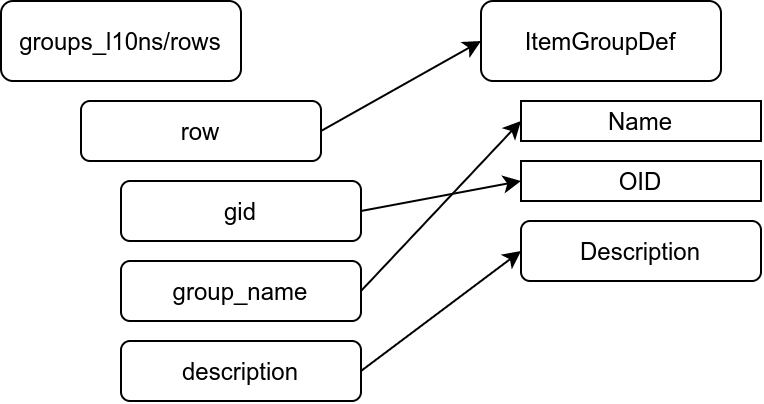
\includegraphics[width=.95\textwidth]{./img/m_groups.png}
			\caption{Mapping der Fragegruppen}
		\end{subfigure}%
		}
		\caption{Diagramme für Fragegruppen und Umfragen}
\end{figure}

\subsection{Fragen}

Grob gesprochen wird die Frage aus LimeSurveys \el{question\_l10ns} Element bei ODM in \el{Question/TranslatedText} der Fragendefinition eingetragen, die Sprache aus \el{language} wird im Attribut \el{xml:lang} eingetragen.
Wie schon bei den Fragegruppen wird die ID übernommen und der Titel wird zum Namen.
Der Hilfstext der Frage wird zur Beschreibung in ODM.
Die Angabe, ob eine Frage verpflichtend ist, kann ebenfalls übernommen werden, allerdigs wird diese in ODM in der Fragen-Referenz eingetragen, nicht in der Definition.

In ODM gibt es allerdings keine Subfragen, dementsprechend muss eine Frage in LimeSurvey potentiell in mehrere Fragen, eine pro Subfrage, umgewandelt werden, damit diese dann in ODM eingefügt werden können.\\

Dementsprechend muss jeder Fragetyp aus LimeSurvey einzeln behandelt werden, wobei die Behandlung eines Fragetyps teils in der Behandlung eines anderen Fragetyps enthalten ist.
Auch sind die Behandlungen für mehrere Fragetypen identisch.
Zum Beispiel werden die Fragetexte der Hauptfrage und der Subfrage konkateniert, um so eine neue Frage  zu formulieren.
Für die Festlegung der \el{OID} von Subfragen wird die \el{qid} der Hauptfrage mit dem Titel der Subfrage konkateniert.
Gründe dafür werden in \cref{im:ans} dargelegt.
Im folgenden werden alle Behandlungen erklärt, mit einer Angabe, für welche Fragetypen diese genutzt werden.

\begin{figure}[h]
			\centering
			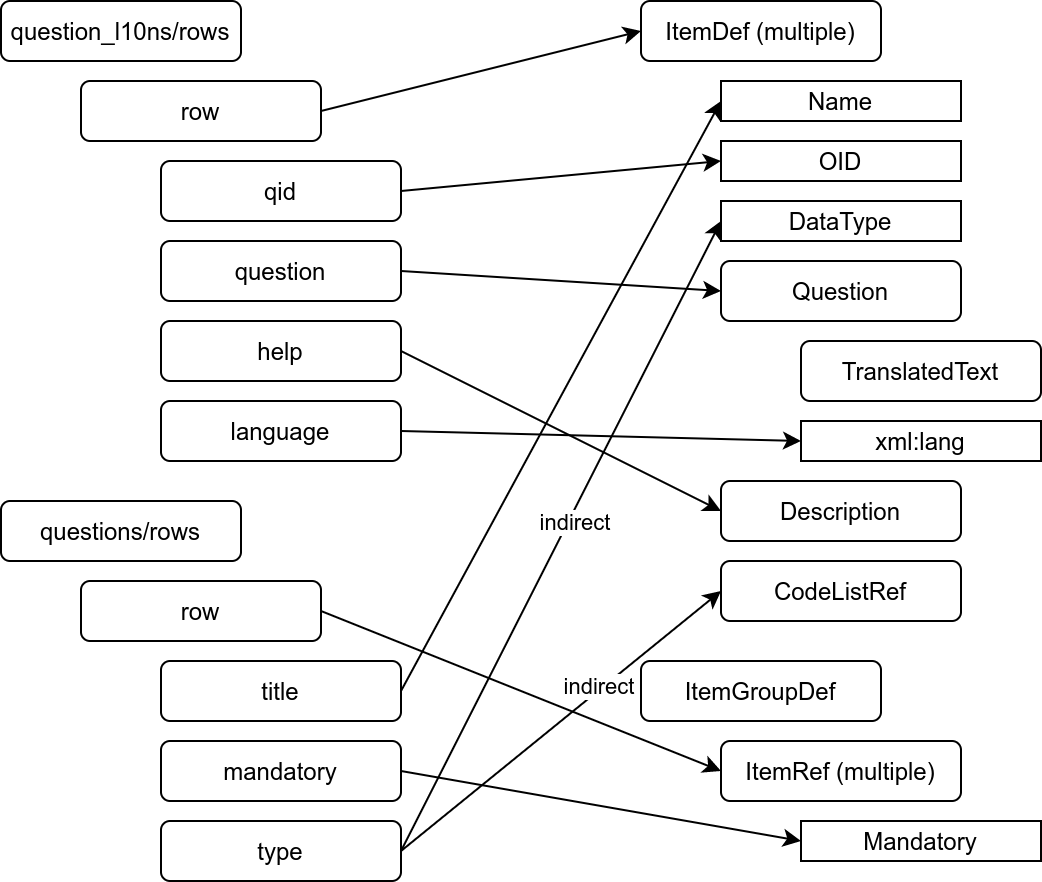
\includegraphics[width=.95\textwidth]{./img/m_questions.png}
			\caption{Mapping der Fragen}
\end{figure}

\subsubsection{Einfachauswahl}
\label{e:sc}

Hier werden die Fragen 1:1 abgebildet, die Antwortmöglichkeiten werden in einer \el{CodeList} gespeichert.
Für den Typ \el{Liste mit Kommentar} wird eine weitere Frage hinzugefügt, deren \el{OID} die \el{qid} der Frage ist, allerdings wird noch \enquote{comment} angehangen.
An den Fragetext wird ebenfalls das gleiche angehangen.
Bei dem Bild der \el{Image-Select-List} besteht das Problem, dass dieses nur mittels Link zum Bild auf dem LimeSurvey-Server eingebettet ist.
Beim Übertragen der Fragen ist somit auch nur dieser Link enthalten.

\subsubsection{Matrix}

Für die Matrizen mit Zahlen- oder Freitextantworten wird eine Frage pro Zelle der Matrix hinzugefügt.
Für alle weiteren Typen dieser Kategorie bis auf die \el{Dual Matrix} wird eine Frage pro Subfrage hinzugefügt, die gleiche Liste an Antwortmöglichkeiten wird für jede Subfrage verwendet.
Die \el{Dual Matrix} wird behandelt, als würde die gleiche Frage zwei Mal mit unterschiedlichen Antwortmöglichkeiten dargestellt.

\subsubsection{Multiple Choice}

Hier wird eine Frage pro Subfrage hinzugefügt, gibt es Kommentare, wird noch eine entsprechende Kommentar-Frage pro Subfrage eingefügt.
Das Bild beim Typ \el{Image Select} wird wie schon bei der Einfachauswahl nur auf Umwegen übernommen.

\subsubsection{Textfragen}

Hier wird der Fragetext wie oben erklärt übertragen, als \el{DataType}-Attribut in \el{ItemDef} wird \enquote{string} gesetzt.
Das funktioniert für alle drei Freitextfragetypen, kurz, lang und riesig so.
Im Falle von \el{Mehrere Texte} wird wieder eine Frage pro Subfrage genutzt.
\el{Input on Demand} und \el{Browser Detect} werden nicht gemappt. Für Details siehe \cref{d:leave}.

\subsubsection{Maskenfragen}

Für den Typ \el{Datum/Zeit} wird der \el{DataType} auf \enquote{datetime} gesetzt.
Für \el{Zahleneingabe} wird der \el{DataType} auf \enquote{float} gesetzt, außer die Option \enquote{Nur Integers} ist angewählt, dann wird stattdessen \enquote{integer} genutzt.
Für \el{Mehrfache Zahlen} wird wieder eine Frage pro Subfrage erstellt.
Für beide Zahlen-Fragen werden Bedingungen, wie den maximalen oder minimalen Antwort-Wert als \el{RangeCheck} übernommen.
Beim Typ \el{Gleichung} handelt es sich nicht um eine Frage, er wird nicht gemappt (siehe \cref{d:leave}).
Es gibt mehrere Typen, bei denen es feste Antwortmöglichkeiten gibt und daher eine CodeList implizit aus dem Typ erstellt wird:
\el{Ja/Nein}, \el{Geschlecht}.
\el{Ranking}, \el{Textanzeige}, \el{Dateiupload} und \el{Sprachumschaltung} werden nicht gemappt. Für weitere Details siehe \cref{d:leave}.

\subsection{Antwortmöglichkeiten}

\begin{figure}[h]
			\centering
			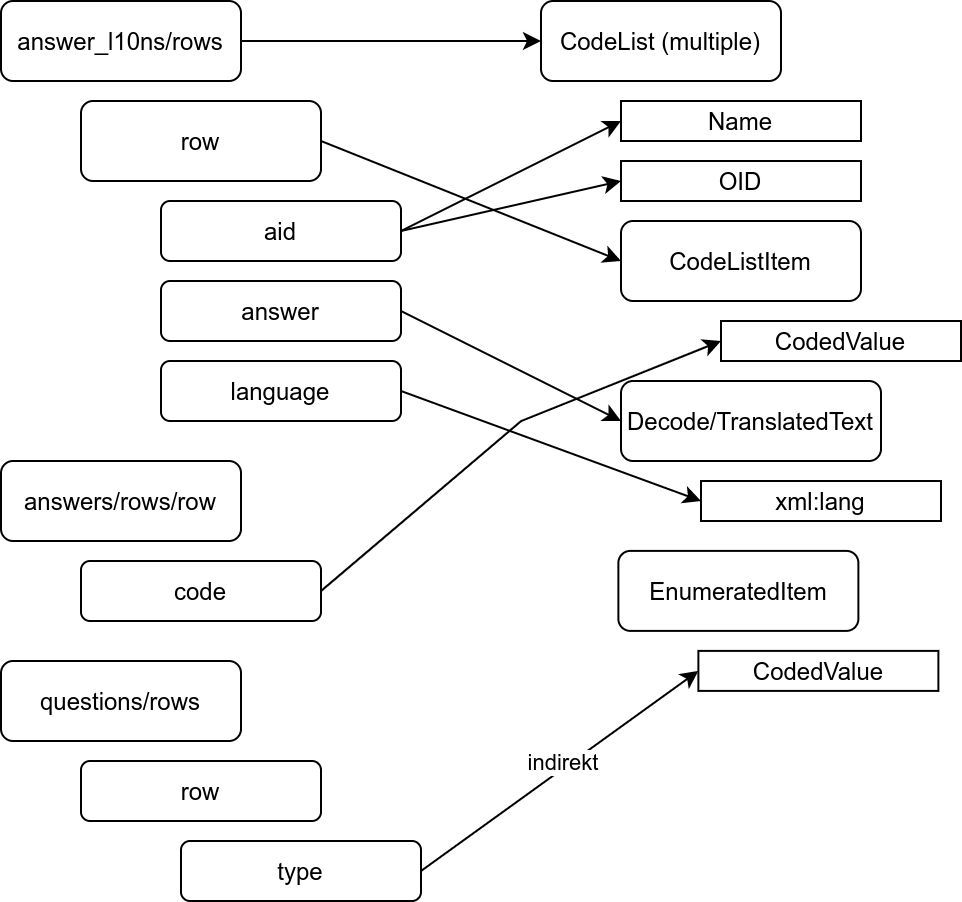
\includegraphics[width=.9\textwidth]{./img/m_answers.png}
			\caption{Mapping der Antwortmöglichkeiten}
\end{figure}

Grundsätzlich wird jedes Mal, wenn es eine vordefinierte Liste an Antwortmöglichkeiten gibt, eine CodeList genutzt, um diese Liste in ODM darzustellen.
Für die Fragen, wo man mit 1 bis 5 oder 1 bis 10 antworten kann, wird eine simple Liste genutzt, für alle weiteren Fragen eine komplexe Liste.
Das liegt unter anderem daran, dass LimeSurvey fast alle Antworten mit einem Buchstaben darstellt und die tatsächlichen Antworten aus mindestens einem Wort bestehen.
So werden komplexere Umwandlungen vermieden und die existierende Struktur wird übernommen.
Für selbstdefinierte Antwortmöglichkeiten ist ohnehin eine komplexe Liste notwendig, da der Ersteller der Umfrage beliebige Kombinationen für Code und Antwort definieren kann.

\subsection{Antworten}

\begin{figure}[h]
	\centering
	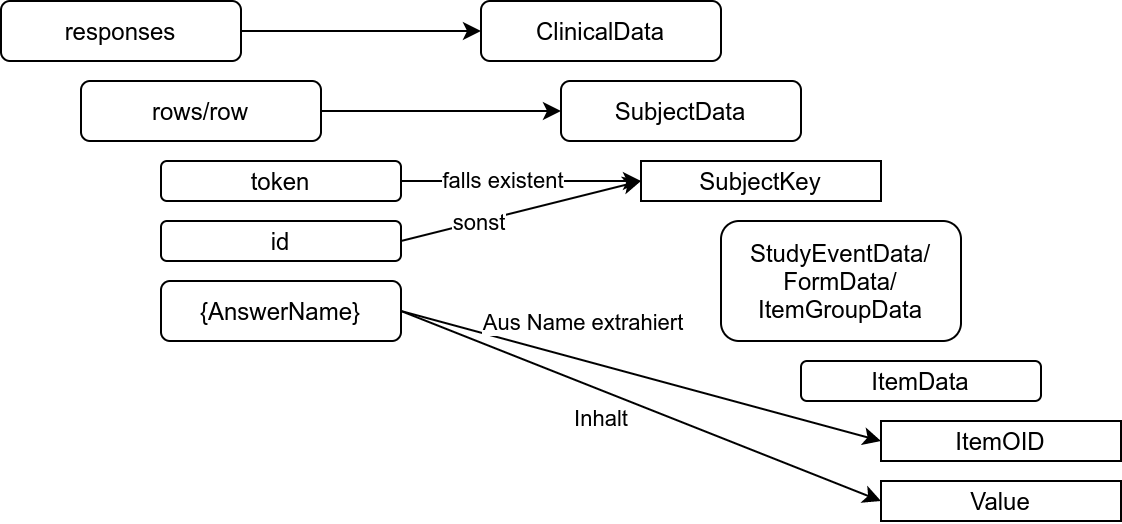
\includegraphics[width=1\textwidth]{./img/m_lsr.png}
	\caption{Mapping des LSR-Formates}
\end{figure}

Als \el{SubjectOID} wird ein Token, falls es ein solches gibt, verwendet. Das liegt daran, dass ein Token pro Teilnehmer eindeutig ist, während es pro Teilnehmer mehrere IDs in LimeSurvey geben kann.
Gibt es kein Token, wird die ID aus LimeSurvey als ID on ODM genutzt.
Ein passender \el{RepeatKey} wird ebenfalls festgelegt, sodass verschiedene Ausfüllungen der Umfrage durch den gleichen Teilnehmer unterschieden werden können.

Als \el{StudyOID} und \el{MetaDataVersionOID} der \el{ClinicalData} werden die entsprechenden OIDs referenziert.
Aus jeder Reihe in LimeSurvey werden hier die Daten eines Teilnehmers gemacht.
Die ID wird übernommen, für die OIDs des \el{StudyEvent's} und des Formulars werden die bereits erstellten Werte eingetragen.
Als ID der Fragegruppe wird die \el{gid} gesetzt.
Als \el{ItemOID} des \el{ItemData} Elements wird ein Teil des Elementnamens genutzt, nämlich \enquote{\{qid\}\{sqid\}\{ext\}}, in \el{Value} wird der Text des Elements eingetragen.
Da die OIDs der Fragen vorher bereits so gewählt wurden, dass sie mit dieser Stuktur übereinstimmen, haben wir bereits funktionierende Referenzen, ohne weitere Umwandlungen vornehmen zu müssen.

\subsection{Themes und Frageattribute}

Die Themes werden nicht in ODM übernommen. Weitere Informationen gibt es in \cref{d:themes}.
Auch von den Frageattributen werden fast keine übernommen, da die meisten der visuellen Darstellung dienen.

\section{Implementierung}

\subsection{Java}

Nun stellt sich die Frage, welche Programmiersprache genutzt werden soll, um den Konverter zu implementieren.
Java bietet sich dabei aus verschiedenen Gründen an.
Einerseits gibt es viele Bibliotheken für Java, welche das Bearbeiten von XML stark vereinfachen, diese Bibliotheken sind auch sehr mächtig und können quasi alles, was man brauchen könnte, um die Aufgabe zu erfüllen.
Darunter sind zum Beispiel Validatoren, die XSD 1.1 unterstützen und Parser, welche mit mehreren Attributen in einem Element umgehen können.
Andererseits wird die Sprache bereits viel am IMI genutzt, der Konverter kann also sehr leicht als JAR in andere Programme eingebunden und von dort aus aufgerufen werden.

\begin{figure}[h]
	\makebox[\linewidth][c]{%
		\begin{subfigure}[b]{.6\textwidth}
			\centering
			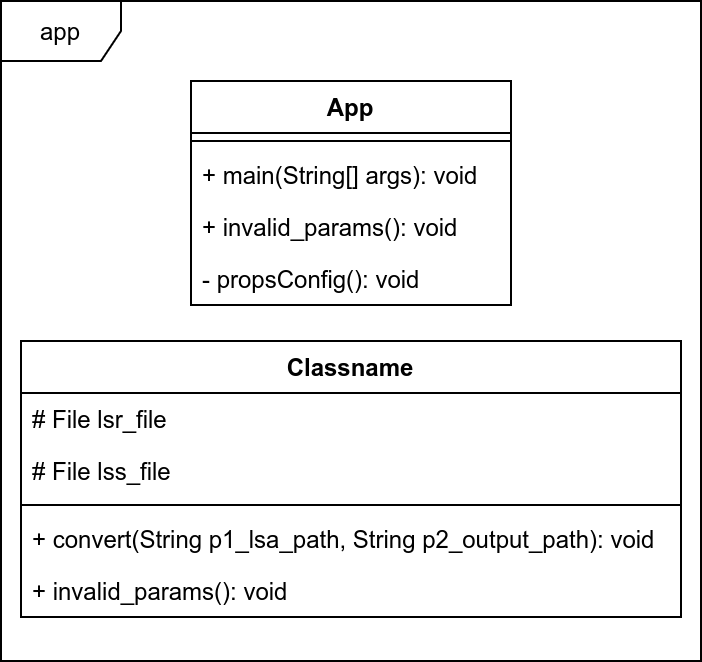
\includegraphics[width=.95\textwidth]{./img/cls_app.png}
			\caption{Klassendiagramm für das Paket \jv{app}}
		\end{subfigure}%
		\begin{subfigure}[b]{.6\textwidth}
			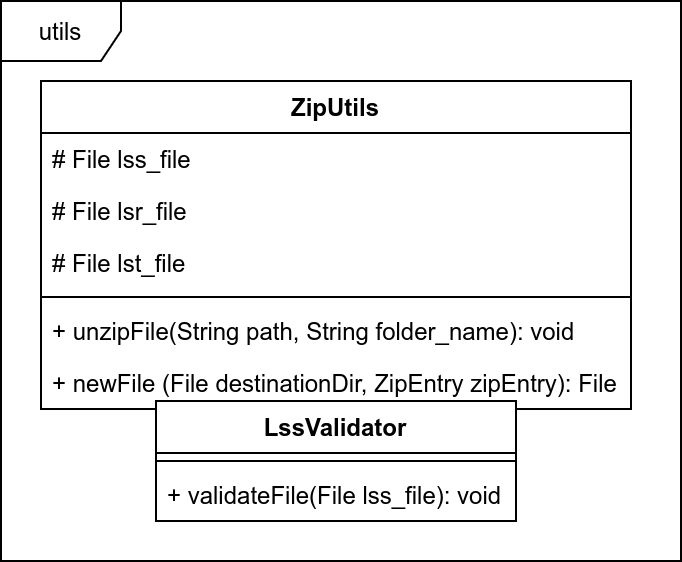
\includegraphics[width=.95\textwidth]{./img/cls_utils.png}
			\caption{Klassendiagramm für das Paket \jv{utils}}
		\end{subfigure}%
		}
		\caption{Klassendiagramme für mehrere Pakete, welche am Anfang der Ausführung gebraucht werden}
\end{figure}

\subsection{Programmaufbau}

Das Programm trägt den Namen \enquote{lsa2odm} und besteht aus vier Paketen, \jv{app}, \jv{utils}, \jv{parser} und \jv{writer}, wobei \jv{parser} in zwei weitere Pakete aufgeteilt ist, \jv{lss} und \jv{lsr}.
in \jv{app} befindet sich die Klasse \jv{App}, welche die \jv{main}-Methode enthält.
Diese erstellt eine Instanz des Konverters \jv{LsaConverter}, auch die Methoden aus \jv{ZipUtils} und \jv{LssValidator} werden hier gebraucht.

\begin{figure}[h]
			\centering
			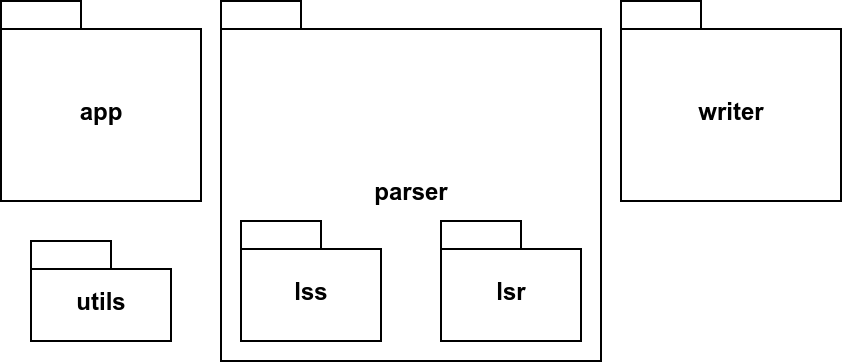
\includegraphics[width=.50\textwidth]{./img/i_package.png}
			\caption{Paketdiagramm für lsa2odm}
\end{figure}

\subsection{Eingabe}

Das Programm erwartet entweder eine oder zwei Eingaben. Der erste Parameter muss dabei der Pfad zum LSA-Archiv sein, der zweite, optionale Parameter ist dabei ein Pfad, wo die ODM-Datei am Ende geschrieben werden soll.
Anschließend wird der erste Parameter mit dem Regulären Ausdruck \enquote{\textasciicircum/?[.*/]*(.*?)\textbackslash\textbackslash.lsa\$} getestet.
Ist der Parameter ein gültiger Pfad zu einer Eingabedatei, wird \jv{unzipFile} auferufen.
Die Funktion beinhaltet relativ generischen Code, welcher ein Zip-Archiv entpackt.
Wenn die Funktion fertig ist, kann man auf alle benötigten Dateien zugreifen und es kann mit den nächsten Aufgaben weiter gemacht werden.

\subsection{Properties}

Es gibt eine Reihe an Strings, welche im Programm gesetzt werden, besonders die Namen der Dummy-Elemente.
Aber auch Suffixe für manche Namen oder der Name der IMI-Syntax ist nicht festgelegt.
Daher sollen all diese Dinge von außerhalb des Codes geändert werden können.
Gibt es noch keine, wird eine Properties-Datei erstellt, welche all diese Informationen beinhaltet.

\subsection{XSD-Validierung}


Das in \cref{an:xsd} erstellte Schema wird nun genutzt, um zu überprüfen, ob die Eingabedatei valide ist.
Das Ergebnis der Prüfung wird dem Nutzer angezeigt, allerdings ist es nicht bindend, auch eine invalide Datei wird konvertiert.
Das liegt vor allem daran, dass sich das Format schnell ändern kann, mehr dazu in \cref{d:version}.
Da diese Änderungen aber oft klein sind, besteht eine hohe Chance, dass der Konverter den Großteil des Dokumentes dennoch verarbeiten kann.
Der Anwender bekommt dennoch die Information, dass der Konverter potentiell nicht mit dieser LimeSurvey-Version funktioniert.

\subsection{Parsing der LimeSurvey Struktur}

Zuerst wird eine Instanz der Klasse \jv{LssParser} mit der entsprechenden LSS-Datei erstellt.
Die Klasse \jv{Survey} dient zum speichern aller gesammelten Informationen, alle für die ODM-Datei benötigten Daten werden hier abgelegt, das Objekt wird später weitergegeben.

Zunächst werden die drei in \cref{a:survey_meta} angesrochenen Elemente mit Metadaten der Studie in die \jv{survey} übernommen.
Dann werden die Fragegruppen übernommen, hierbei werden alle für das Mapping relevante Informationen gespeichert.

\begin{figure}[h]
	\label{im:fig:lss}
			\centering
			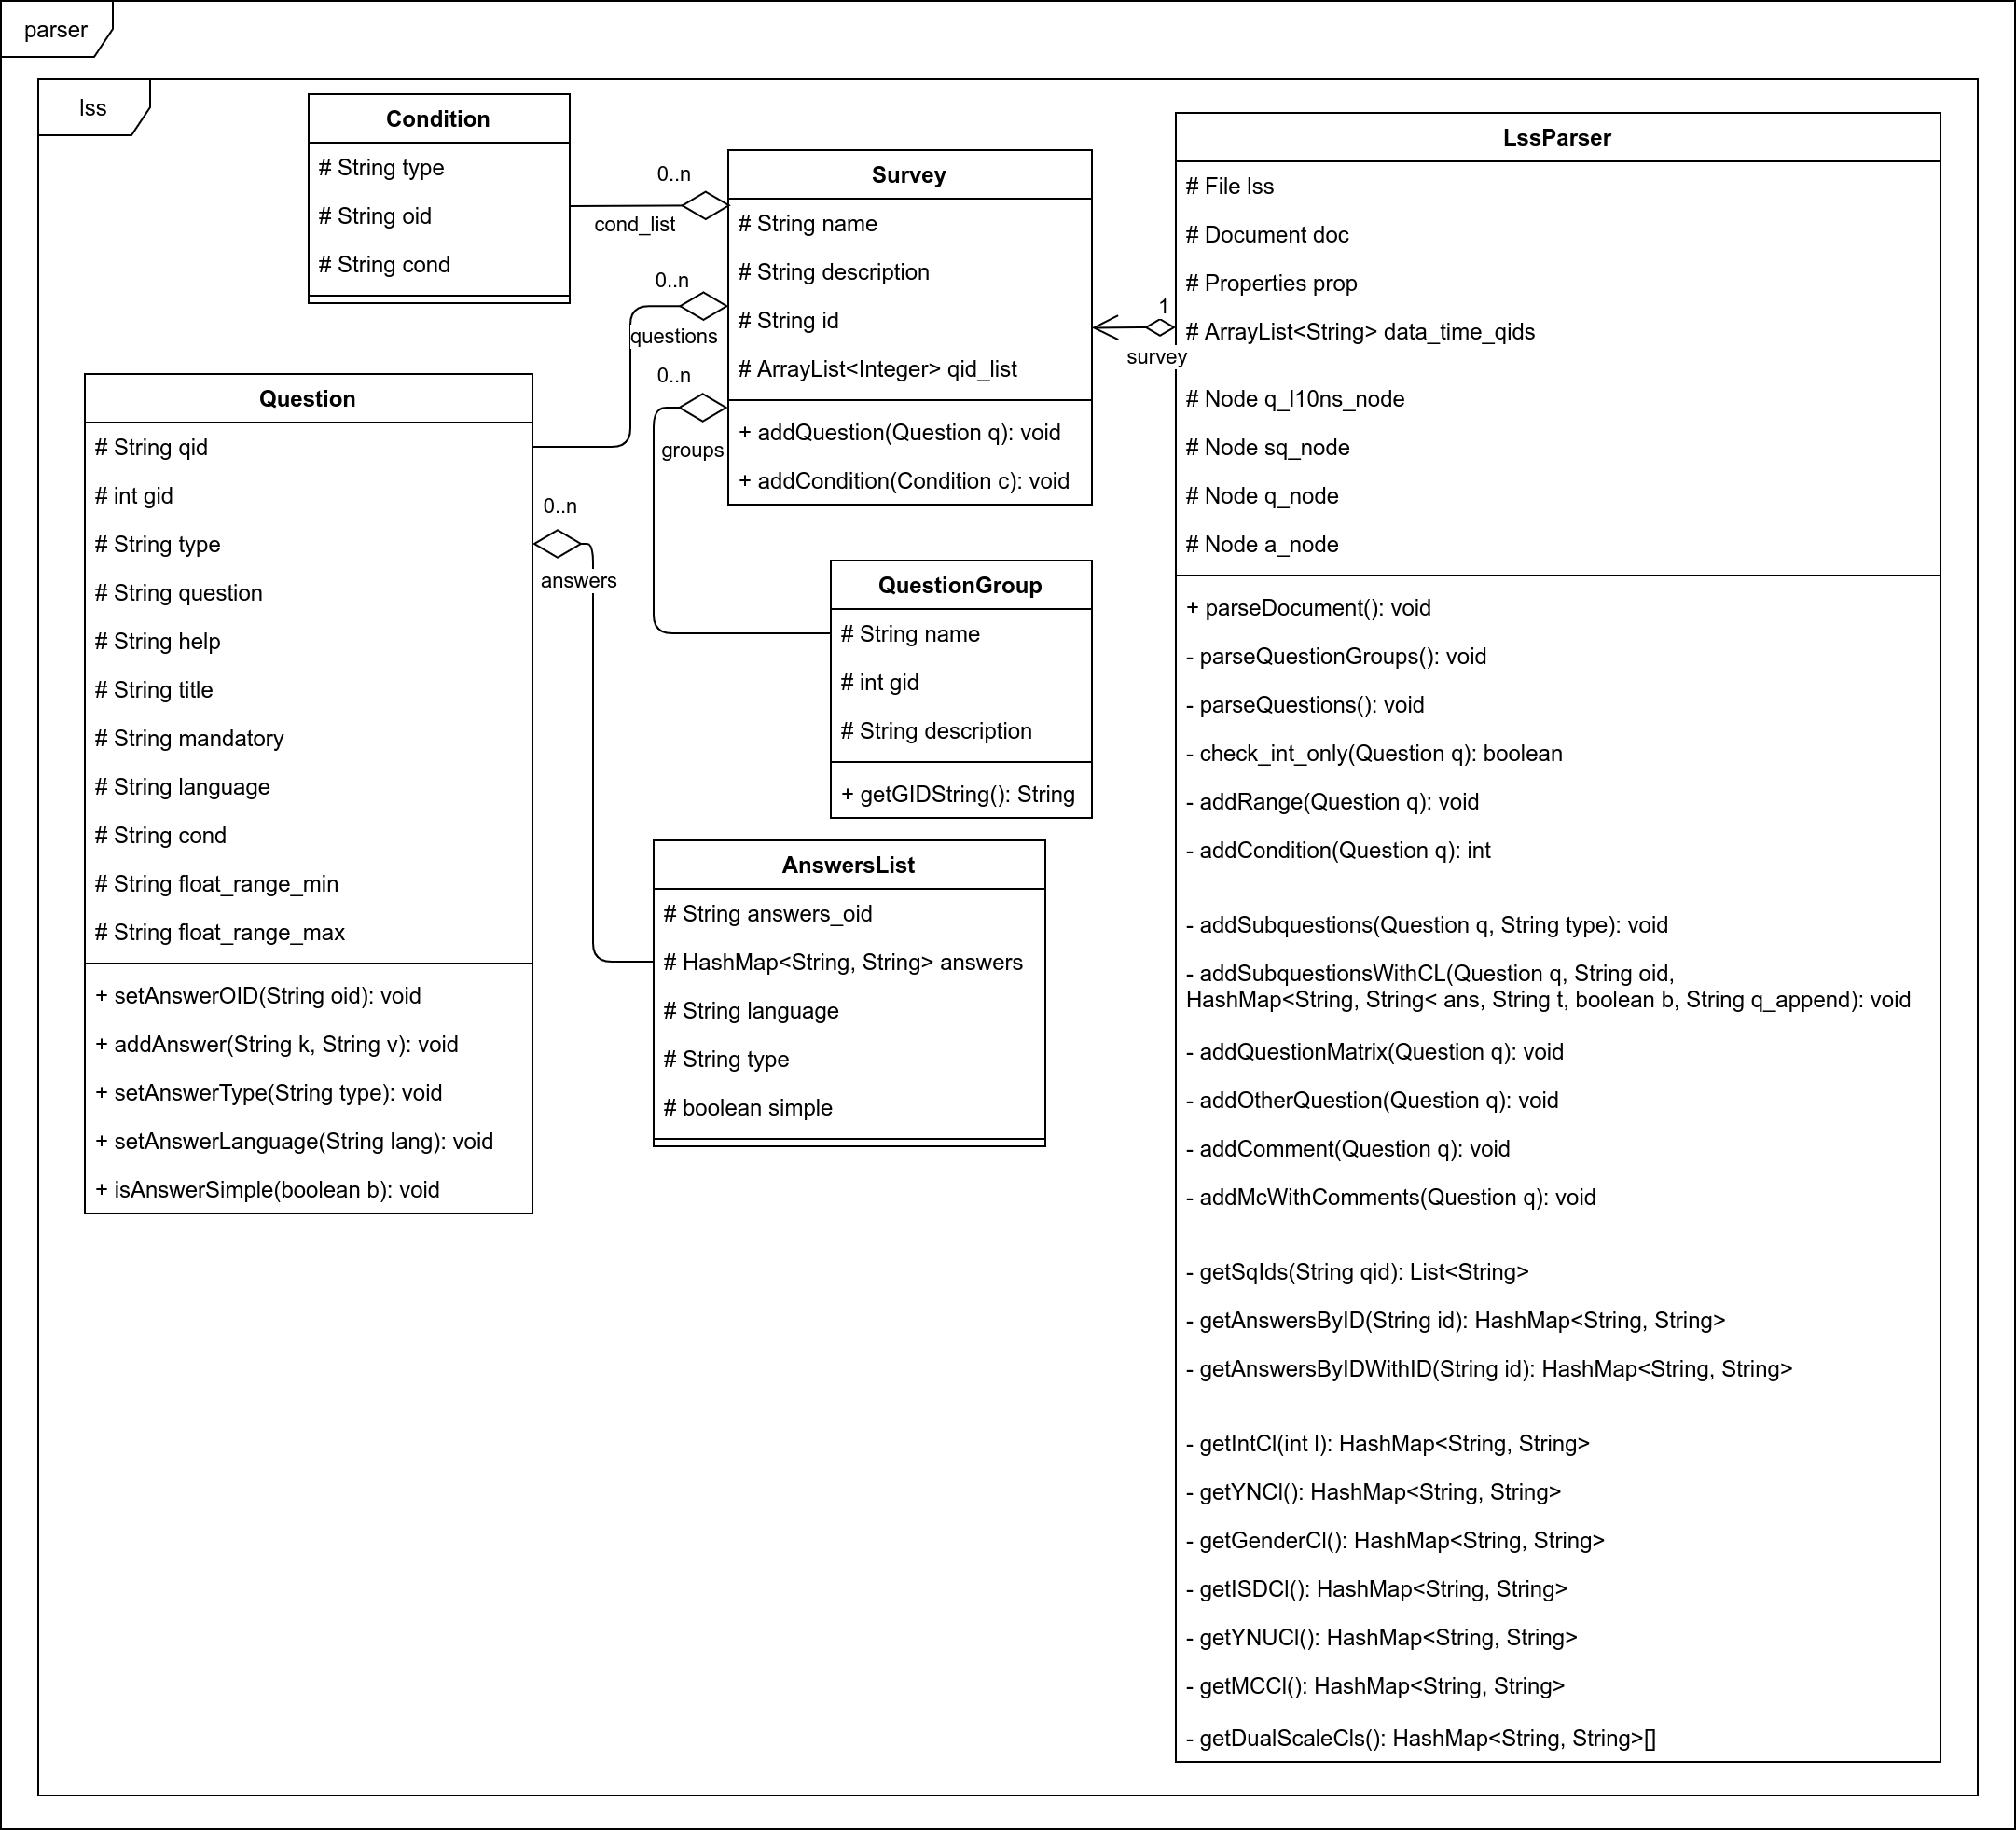
\includegraphics[width=0.99\textwidth]{./img/cls_lss.png}
			\caption{Klassendiagramm für das Paket \textit{lss}}
\end{figure}

\subsubsection{Parsing der Fragen}
\label{im:q}

Als nächstes werden die Fragen in \jv{survey} übernommen. Dabei werden diese bereits gemäß des Mappings umgewandelt.
Das wird gemacht, um die Gesamtstruktur so früh wie möglich zu simplifizieren und nicht für jede Frage eine gesonderte Klasse erstellen zu müssen.
Da sich viele Fragen im Aufbau stark ähneln, ist dies ein simpler und schneller Weg, das Ziel zu erreichen.
Am Ende dieser Verarbeitung soll es noch vier Fragetypen geben:

\begin{enumerate}[leftmargin=0.5cm]
\item[T] Eine Frage, auf die mit einem Freitext geantwortet werden kann
\item[N] Bei dieser Frage muss mit einer Zahl im float-Format geantwortet werden
\item[I] Bei dieser Frage muss mit einer Zahl im integer-Format geantwortet werden
\item[A] Bei dieser Frage muss aus einer vordifinierten Liste an Antwortmöglichkeiten gewählt werden
\item[D] Diese Frage hat ein Datum und eine Uhrzeit als Antwort
\end{enumerate}

Zuerst wird eine Liste aller \el{row} Elemente des Frage-Elements erstellt, durch welche im Anschluss iteriert wird.
Die Klasse \jv{Question} soll alle Informationen über eine Frage speichern, entsprechend wird diese genutzt, um die Informationen jeder Reihe zu speichern.
Eine Liste der Daten ist in \cref{im:fig:lss} zu sehen.
Nicht in jedem Fall wird diese Frage auch zur Umfrage hinzugefügt, wenn es sich zum Beispiel um eine Matrix-Frage handelt, wird diese Instanz nur zum Erstellen neuer Fragen genutzt.
Dann werden potentiell existierende Bedingungen hinzugefügt, dieser Vorgang wird in \cref{im:cond} beschrieben.

Anschließend gibt es ein \jv{switch}-Statement, welches einen passenden Weg zum Parsen der Frage abhängig vom Typ ausführt.

\subsubsection{Textfragen}
Für Textfragen wird hier nur der Typ geändert, sodass alle Arten von Textfragen \enquote{T} als Typ haben.

\subsubsection{Datum/Zeit}
Bei Datum/Zeit-Fragen wird die \el{qid} zu einer Liste hinzugefügt, welche später in \cref{im:ans} gebraucht wird.

\subsubsection{Numerische Eingaben}
Wenn es sich um eine Frage mit numerischer Antwort handelt, wird geprüft, ob die Antwort nur ganzzahlige Werte enthalten darf. In dem Fall wird der Typ auf \enquote{I} gesetzt. 
Dann wird überprüft, ob es Minimal- und Maximalwerte für die Antwort gibt, wenn ja werden entsprechende Werte in der Frage-Klasse gesetzt.

\subsubsection{Listen}
Handelt es sich um eine Frage vom Typ \el{Liste mit Kommentar}, wird zuerst eine weitere Frage hinzugefügt, welche den Kommentar speichern soll.
Dann wird mit der Behandlung für die anderen \el{Listen}-Fragen fortgefahren.
Bei selbiger wird geschaut, ob die Option für \jv{Anderes} aktiviert ist, wenn ja, wird auch dafür eine Frage hinzugefügt.
Dann wird eine Liste mit Antwortmöglichkeiten an die eigentliche Frage angehangen und selbige wird hinzugefügt.

\subsubsection{Restliche Einfachauswahl}
Für die Fragetypen \el{Fünf Punkte Auswahl}, \el{Ja/Nein} und \el{Geschlecht} wird der Typ geändert und eine entsprechende Antwort-Liste mittels der dafür erstellten Hilfsfunktionen generiert.

\subsubsection{Multiple Antworten}

Wird nach Zahlen verlangt, werden erst potentielle Constraints ermittelt und hinzugefügt, dann wird der Typ angepasst, je nach Gleitkomma- oder Ganzzahl-Antworten.
Dann wird bei beiden die Funktion \jv{addSubquestions} aufgerufen.
Diese sucht die IDs aller Subfragen und fügt dann entsprechende Kopien der Hauptfrage ein, Änderungen werden wie oben beschrieben durchgeführt.

\subsubsection{Duale Skalen}

Geht es um diesen Typ, werden erst beide Listen mit Antworten angelegt, dann wird die Funktion \jv{addSubquestionsWithCL} zwei Mal aufgerufen, einmal mit jeder Skala.
Beim ersten Mal wird \enquote{-0} an die Frage-ID angehangen, beim zweiten Mal \enquote{-1}.

\subsubsection{Matrizen (Text, Numerisch)}

In beiden Fällen werden hier die Antwortmöglichkeiten auf den Achsen gesammelt, dann wird für jede Kombination eine neue Frage erstellt, der Inhalt wird angepasst.

\subsubsection{Arrays}

Für alle Array-Fragen wird die Funktion \jv{addSubquestionWithCL} aufgerufen, die Liste an Antworten, deren Name un der Datentyp wird jeweils angepasst.

\subsubsection{Mehrfachauswahl}

Hier werden auch alle Subfragen mit einer Antwortliste eingefügt, die Liste enthält \enquote{Y} für Ja und énquote{} für Nein.
Dann wird noch eine potentielle \jv{Anderes}-Frage eingefügt.
Hat die Auswahl noch Kommentare, wird eine spezielle Funktion aufgerufen.
Diese hat fsat gleichen Inhalt, allerdings wird noch ein Kommentar für jede Frage eingefügt.
Eine passende Bedingung wird auch eingefügt, sodass die Kommentar-Frage nur angezeigt wird, wenn die Möglichkeit auch ausgewählt wurde.

Dabei wird die Frage-ID wie folgt aufgebaut: \enquote{\{Parent\_QID\} + \{Title(y-Axis)\}\_\{Title(x-Axis)\}}.

\subsubsection{Parsing der Anzeige-Bedingungen}
\label{im:cond}

Da die Bedingungen innerhalb des LSS-Formates ohnehin als Elemente gespeichert werden und nicht als ExpressionScript, ergibt es mehr Sinn, diese nicht wieder in ExpressionScript umzuwandeln, sondern direkt in die Syntax des IMI.
Die in LimeSurvey mit ExpressionScript formulierten Bedingungen geben an, wann eine Frage angezeigt werden soll.
Die in ODM definierten Bedingungen müssen zu \enquote{True} evaluieren, wenn eine Frage nicht angezeigt werden soll.
Der fertige Ausruck muss am Ende also negiert werden.
Dann werden alle Bedingungen rausgesucht, welche zur \el{qid} gehören.
Diese sollen nun durch ein logisches \enquote{Und} verknüpft werden.

Die Frage aus \el{cfieldname} wird mittels des regulären Ausdrucks
\reg{\textasciicircum\textbackslash\textbackslash d+X(\textbackslash\textbackslash d+)X(.+?)\$}
\noindent so verarbeitet, dass wir die darin enthaltene \el{gid} und \el{qid} der Frage enthalten.
Mit diesen, der Dummy-ID für das \jv{StudyEvent} und der Umfragen-ID wird dann ein Pfad gemäß der IMI-Syntax erstellt.

Handelt es sich nicht um einen Regulären Ausdruck, der als Operator genutzt wird, werden folgende drei Teile in dieser Reihenfolge aneinander gehangen: 
\reg{\{PATH\} \{OPERATOR\} \{VALUE\}}
\noindent wobei das Element \el{method} den Operator enthält und \el{value} den Wert. \jv{PATH} ist der vorher erstellte Pfad.

Handelt es sich um einen regulären Ausdruck, wird das führende Leerzeichen entfernt und die Bedingung in folgender Form aufgeschrieben:
\reg{MATCH(\{REGEX\}, \{PATH\})}

Soll eine Antwort leer bleiben, wird \enquote{NULL} als Wert verwendet.
Bei beidem handelt es sich nicht um einen Teil der IMI-Syntax, weiteres dazu in \cref{d:imi}.

Abschließend wird der Bedingung eine OID der Form \el{\{qid\}\{ex\}} gegeben, wobei \el{ex} in der Properties-Datei festgelegt werden kann.
Diese wird auch in der Frage eingetragen, damit man später eine Referenz auf die Bedingung hat.

\subsection{Parsing der LimeSurvey Antworten}
\label{im:ans}

Die Klasse \jv{LsrParser}, zusammen mit den Klassen \jv{Response} und \jv{Answer} wurde erstellt, um die Antworten zu verarbeiten.
Zuerst wird in \jv{createDocument} ein neuer SAXReader erstellt, welcher die LSR-Datei in eine Instanz der Klasse \jv{Document} einliest.
Selbige wird dann in \jv{parseAnswers} weiterverwendet.

\begin{figure}[h]
			\centering
			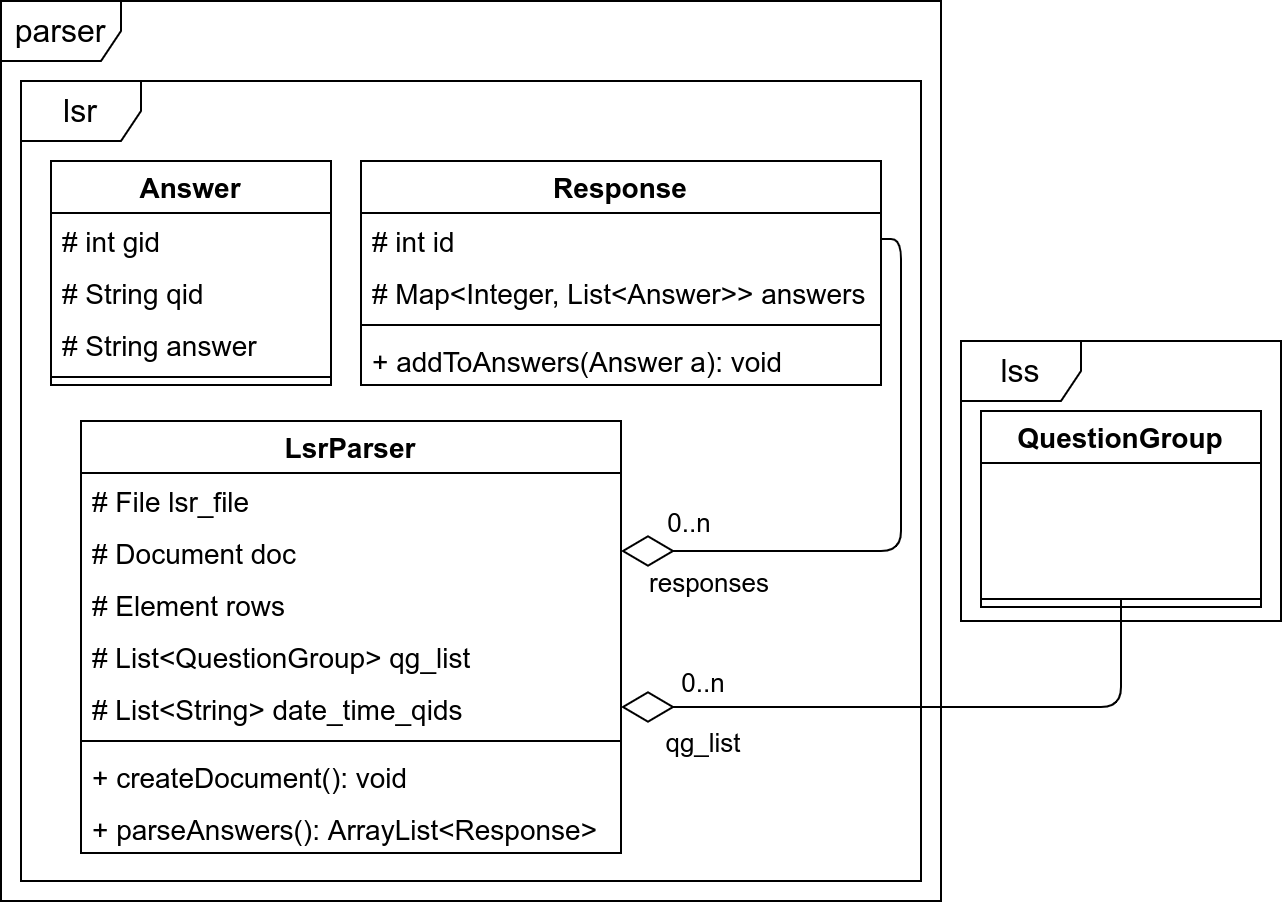
\includegraphics[width=.98\textwidth]{./img/cls_lsr.png}
			\caption{Klassendiagramm des Paketes \textit{lsr}}
\end{figure}

Alle für das Parsing relevanten Felder stehen in \el{document/responses/rows}. Dort gibt es eine Reihe pro Beantwortung des Fragebogens.
Die Klasse \jv{Response} dient zum Speichern einer Reihe, daher werden Instanzen erstellt, um alle Informationen der LSR-Datei zu übertragen.
Als nächstes wird über alle Kind-Elemente der Reihe iteriert und es wird nach Antworten gesucht.
Diese sind an der Struktur des Element-Namens zu erkennen, sie besitzen fast den gleichen Aufbau wie der Inhalt des Elements \el{cfieldname} aus \cref{im:cond}, allerdings gibt es hier zusätzlich noch einen führenden Unterstrich.
Wir nutzen also den regulären Ausdruck \enquote{\textasciicircum\textunderscore\textbackslash\textbackslash d+X(\textbackslash\textbackslash d+)X(.+?)\$}, um pasende Elemente zu finden und mittels der Capture Groups die \jv{gid} und \jv{qid} zu erhalten.

Dann wird geprüft, ob die Antwort leer ist, in dem Fall wird sie ignoriert.
Ist sie nicht leer, wird geschaut, ob es sich um eine \el{Datum/Zeit} Frage handelt, dazu wird die in \cref{im:q} erstellte Liste genutzt. Dies ist notwendig, damit das Format dem Datentyp \enquote{xsd:dateTime} entspricht, welcher später gefordert wird.
Anschließend wird eine neue Instanz der Klasse \jv{Answer} erstellt, diese soll die Antwort auf eine Frage sichern.
Befüllt wird sie mit den vorher gewonnenen Informationen über die Frage.


Schließlich wird die Antwort mittels der Methode \jv{addToAnswers} zu \jv{answers} hinzugefügt.
Diese Methode sortiert die Antwort dabei passend ein, sodass am Ende alle Antworten zu Fragen aus der gleichen Fragegruppe in einer Liste sind.

Dann wird die \jv{Response} in die ensprechende Liste hinzugefügt.
Als Teil des Objektes \jv{survey} wird sie später an den \jv{ODMWriter} weitergegeben, damit die Antworten dort übertragen werden können.

\subsection{Ausgabe als ODM-Datei}

Mittels der Klasse \jv{ODMWriter} soll eine neue ODM-Datei erstellt werden. Der Konstruktor nimmt dabei die beim Parsing erstellte \jv{Survey} entgegen.
Die Methode \jv{createODMFile} dient vor allem als Caller für andere Methoden, welche die eigentlichen Funktionen ausführen.

\subsubsection{Studienstruktur}

Zuerst erstellt \jv{createODMRoot} das Wurzelelement \el{ODM} mit allen benötigten Attributen.
Als nächstes wird \jv{addStudyData} aufgerufen. Hier werden die Elemente \el{Study}, sowie die globalen Variablen mittels der Dummy-Werte aus der Properties-Datei erstellt.
Weiterhin werden die Elemente \el{MetaDataVersion},\el{Protocol}, \el{StudyEventDef} und \el{Form} erstellt, alle relevanten oder benötigten Attributewerte werden gesetzt.
Die \jv{meta\_data\_oid} besteht dabei aus dem Prefix in der Properties-Datei und der Studien-ID.
Die Attributwerte für die \el{StudyEventDef} stammen aus der Properties-Datei, das Formular wird gemäß des Mappings befüllt.

\subsubsection{Fragetypen}

Nun werden die Fragegruppen mittels \jv{addQuestionGroups} hinzugefügt. Wie in \cref{m:qg} beschrieben wird aus jeder Fragegruppe eine \el{ItemGroupDef}.
Im Formular wird die entsprechende Referenz auf die Fragegruppe eingefügt.
Gibt es eine Beschreibung, wird sie in eine Beschreibung in der \el{ItemGroupDef} eingefügt.
Die Fragen brauchen später Referenzen in den Fragegruppen, daher werden Referenzen auf alle Fragegruppen gespeichert, sodass man später einfach Elemente hinzufügen kann.

\begin{figure}[h]
	\centering
	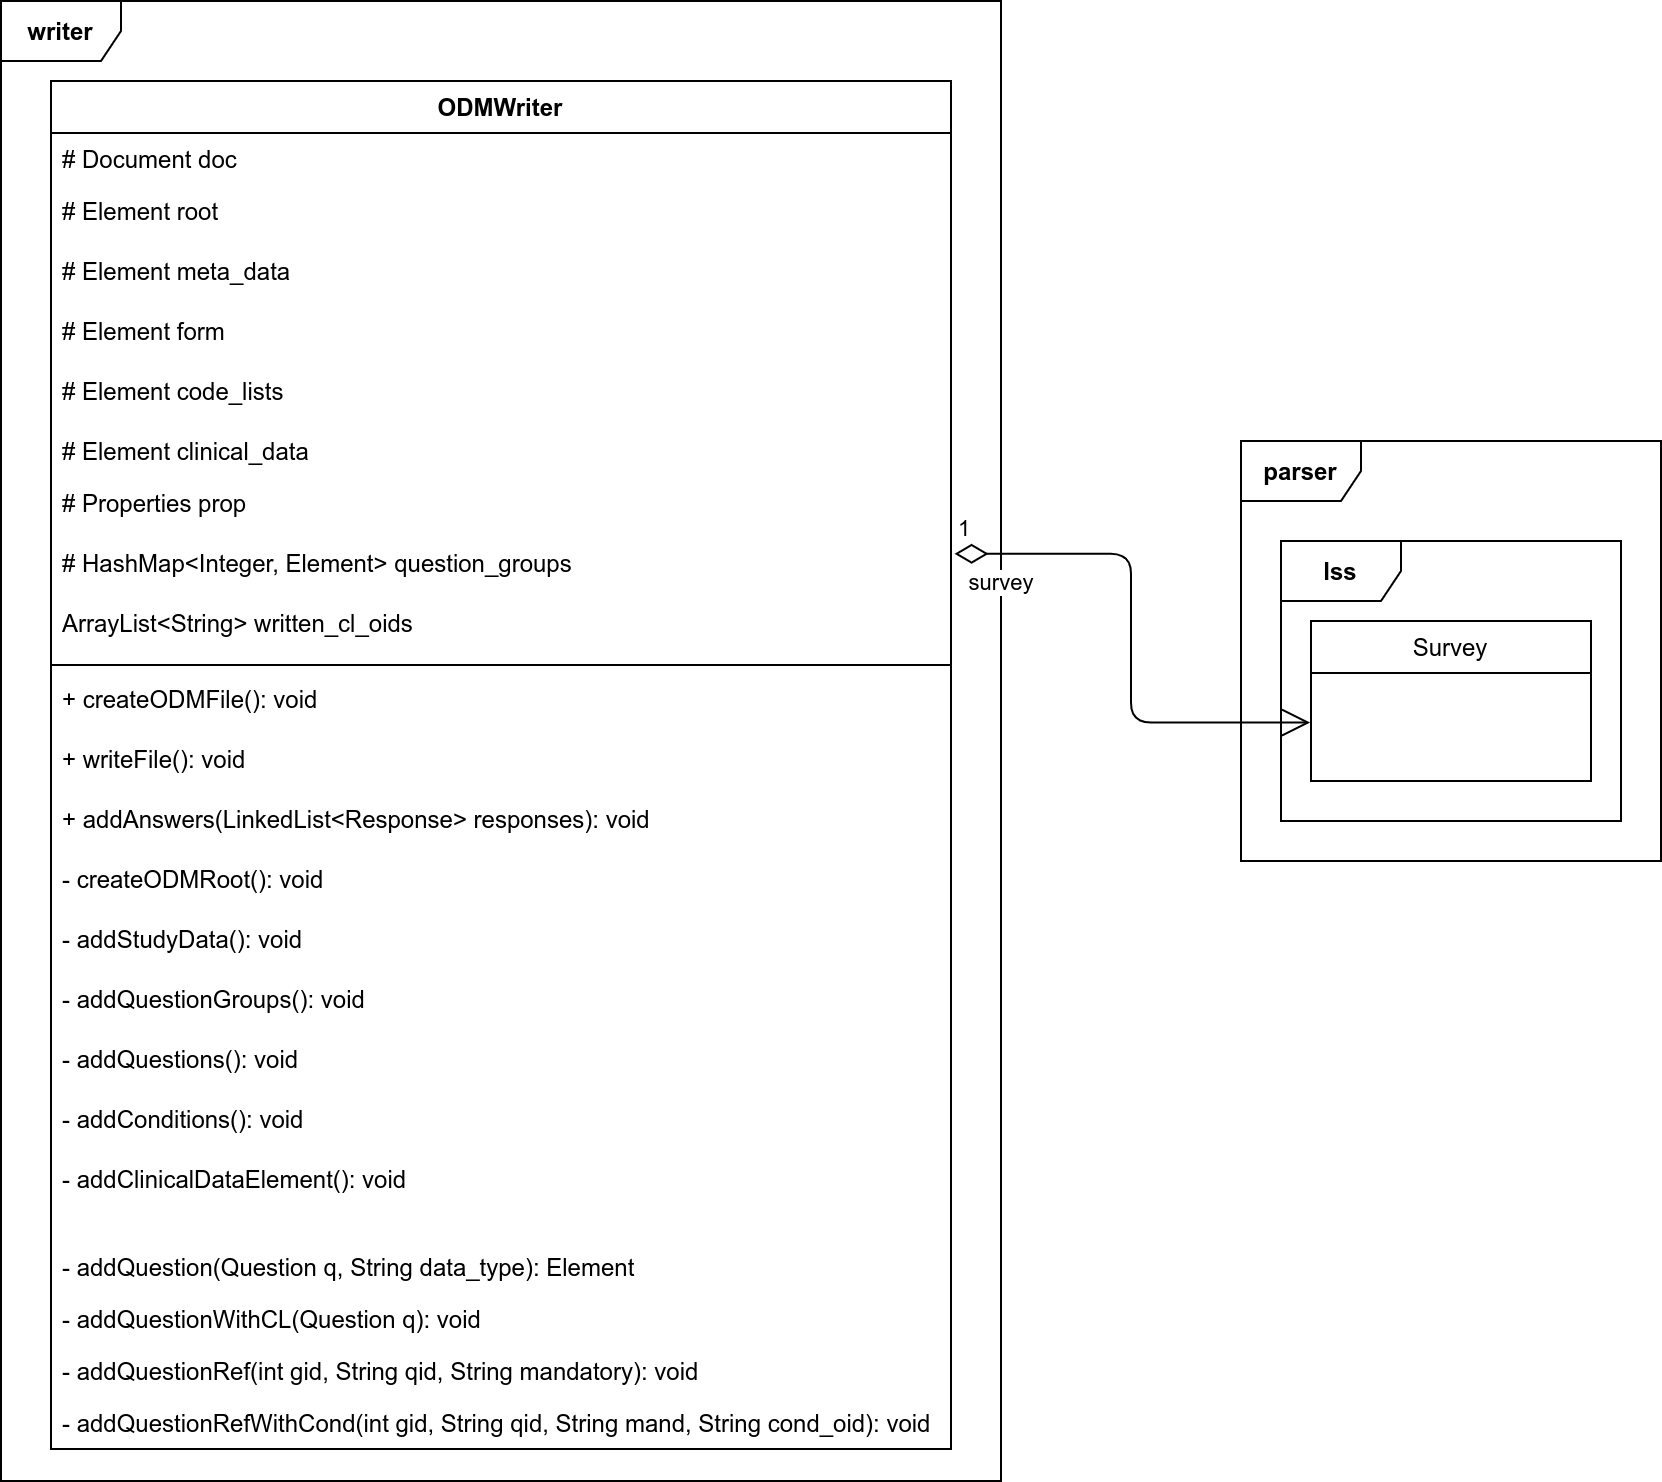
\includegraphics[width=.98\textwidth]{./img/cls_writer.png}
	\caption{Klassendiagramm des Pakets writer}
\end{figure}

\subsubsection{Fragen}

Danach werden alle Fragen in der Methode \jv{addQuestions} eingefügt.
Zuerst wird ein zweites Dokument mit einem Wurzelelement erstellt, um alle \el{CodeList} Elemente zu speichern.
Dies wird gemacht, da die Listen mit den Antworten hinter allen Fragen stehen sollen, eine Frage zwischen der letzten Frage und der ersten Antwortliste einzufügen ist allerdings nicht unbedingt einfach.
Theoretisch kann man mittels der Methode \jv{add} einen Index angeben und so ein Element an einer beliebigen Stelle einfügen.
Da sich der Index hier allerdings mit jedem Einfügen einer neuen Frage verändert, ist es simpler, die Listen einfach erst auszulagern und später mit \jv{appendContent} einfach alle Elemente zu übertragen.

Anschließend wird über den Typ entschieden, welche Methode zum Einfügen der Frage aufgerufen wird. Dabei gibt es hier nur noch die fünf Typen, auf welche alle Fragen in \cref{im:q} reduziert wurden.
Bei einer Array-Frage wird \jv{addQuestionWithCL} aufgerufen, was die Frage und die Antwortliste einfügt.
In allen anderen Fällen wird \jv{addQuestion} aufgerufen, der übergebene Datentyp variiert dabei entsprechend.
Zuletzt wreden alle Antwortlisten übertragen.

\subsubsection{Klinische Daten}

Zuerst muss das Element für Klinische Daten im Wurzelelement erstellt werden.
Anschließend ist \jv{createODMFile} fertig, die Antworten werden jetzt durch eine öffentliche Methode hinzugefügt.
Diese wird im LSR-Parser aufgerufen, die Rationale dafür wurde bereits in \cref{im:ans} erklärt.

\subsubsection{Ausgabe}

Mittels \jv{writeFile} wird nun das vorher erstellte Dokument geschrieben.
Der Name der Ausgabe-Datei ist \enquote{\{Survey-ID\}.xml}, sie wird am Ausgabepfad geschrieben, falls einer angegeben wurde.
Zusätzlich wird das Dokument formatiert, sodass es auch von Hand lesbar ist. Dazu reicht in \jv{dom4j}
\[OutputFormat format = OutputFormat.createPrettyPrint();\]
Das erstellte Format kann dann an den \jv{XMLWriter} gegeben werden.

% Dieses Kapitel sollte die Ergebnisse beinhalten, die mit den Methoden aus \autoref{ch:methodik} erstellt wurden.

% \begin{table}[h]
% \caption{Beispieltabelle}
% \begin{center}
% 	\begin{tabular}{|c||c|c|}
% 		\hline
% 		Spalte1 & Spalte2 & Spalte3 \\
% 		\hline\hline
% 		   1    &    2    &    3    \\
% 		\hline
% 	\end{tabular}
% \end{center}
% \label{tbl:table}
% \end{table}
